\chapter{Grundlagen und Stand der Technik}
\label{sec.Grundlagen und Stand der Technik}

In diesem Kapitel wird der aktuelle Stand der Technik zu Methoden der binären sowie quantitativen Darstellung von Umweltzuständen präsentiert. Es werden die mathematischen Grundlagen der in dieser Arbeit verwendeten Methoden behandelt. Neben Fourierreihen (Abschnitt \ref{sec.Fourierreihen und Fouriertransformation}) und der diskreten Fouriertransformation (Abschnitt \ref{sec.Diskrete Fouriertransformation}) wird  außerdem auf die Thematik der Wahrscheinlichkeitsverteilungen eingegangen. Aufgeführt wird neben der Binomialverteilung auch die Poissonverteilung (Abschnitt \ref{sec.Poissonverteilung}). \\
Darauf folgend werden Ergebnisse der Wissenschaft zur Beschreibung von Zustandsmodellen vorgestellt. Während Abschnitt \ref{sec.Beschreibung binärer Zustandsmodelle} sich mit der Beschreibung binärer Zustandsmodelle beschäftigt, legt Abschnitt \ref{sec.Beschreibung quantitativer Zustandsmodelle} den Fokus auf die Beschreibung quantitativer Zustandsmodelle. 

\section{Fourierreihen und Fouriertransformation}
\label{sec.Fourierreihen und Fouriertransformation}
Periodische Signale tauchen in vielen Bereichen der Physik und Technik auf. Ein Signal bezeichnet hierbei eine Funktion, welche eine physikalische Größe in Abhängigkeit von der Zeit, dem Ort, oder einer anderen Variablen darstellt \cite{Eichler.2006}. Betrachtet man periodische Funktionen, so zeichnen sich diese durch ihre Periodendauer $T$ aus. Eine Periode enthält dabei die gesamte Information des Signals, sodass gilt: $f(t) = f(t+T)$. Jede periodische Funktion kann durch eine Überlagerung von Sinus- und Kosinusfunktionen unterschiedlicher Periodendauern $2 \pi n$ approximiert werden \cite{Eichler.2006}. Dargestellt werden kann dies durch eine Fourierreihe 

\begin{equation}
	\label{eq:Fourierreihe}
	f(t) = \dfrac{a_0}{2} + \sum_{n=0}^N[a_n \cos(n \omega t) + b_n \sin(n \omega t)].
\end{equation}
Hierbei bezeichnet $\omega = 2 \pi / T$ die Kreisfrequenz der Grundschwingung. Die Konstanten $a_0,a_1 \dots a_n$ werden als gerade Fourierkoeffizienten bezeichnet, $b_1, b_2 \dots b_n$ hingegen als ungerade Fourierkoeffizienten. Dies leitet sich daraus ab, dass der Cosinus eine gerade und der Sinus eine ungerade Funktion ist. \\
Alternativ lässt sich eine Fourierreihe durch Sinusfunktionen mit unterschiedlichen Amplituden und Phasen beschreiben. Die Fourierreihe lautet dann
\begin{equation}
	\label{eq:Fourierreihe_umgerechnet}
	f(t) = \rho_0 + \sum_{n=1}^{N} \rho_n \sin(n \omega t + \varphi_n).
\end{equation}
Die Grundfrequenz des Signals lautet $f_1 = 1/ T = \omega / 2 \pi$. Die weiteren Sinus- und Kosinusfunktionen der Fourierreihe besitzen Frequenzen $f_n = nf_1$, also ganzzahlige Vielfache der Grundfrequenz. Die Umrechnung von Gleichung \ref{eq:Fourierreihe} nach Gleichung \ref{eq:Fourierreihe_umgerechnet} erfolgt mithilfe der Definitionen
\begin{equation}
	\label{eq:rho_0} 
	\rho_0 = \frac{a_0}{2} ,
\end{equation}
\begin{equation}
	\label{eq:rho_n}
	\rho_n = \sqrt{a_n^2 + b_n^2} ,
\end{equation}
\begin{equation}
	\label{eq:phi_n}
	\varphi_n = \arctan(\frac{a_n}{b_n}) .
\end{equation}
Mit $\rho_0$ wird hierbei der Gleichanteil des Signals bezeichnet, $\rho_n$ steht für die Amplitude der \textit{n}-ten Frequenz und $\varphi_n$ für die Phasenverschiebung der \textit{n}-ten Frequenz \cite{Eichler.2006}. Ein Signal kann also durch sein Kosinus- und Sinusspektrum sowie durch sein Amplituden- und Phasenspektrum charakterisiert werden. 
Grafisch veranschaulicht wird die Fourierreihe durch \bild{Fourier}. In Bild \ref{fig.Fourier_a} eingezeichnet ist ein periodisches Signal mit der Periodendauer $T$, für welches $f(t) = f(t + T)$ gilt. In Bild \ref{fig.Fourier_b} finden sich die das Gesamtsignal definierenden Frequenzen, mit ihren zugehörigen Amplituden $\rho$ und Phasenversätzen $\varphi$ \cite{Eichler.2006}.
\begin{figure}[!ht]
	\centering
	\subfigure[Periodisches Signal $F(t) = F(t + T $\label{fig.Fourier_a})]{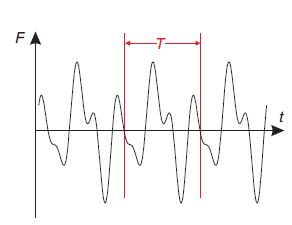
\includegraphics[height=50mm]{Abbildungen/grundlagen/signal}}
	\hspace{5mm}
	\subfigure[Amplituden- und Phasenspektrum des Signals\label{fig.Fourier_b}]{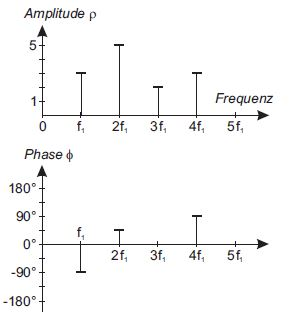
\includegraphics[height=50mm]{Abbildungen/grundlagen/amplituden_phasenspektrum}}
	\caption{Periodisches Signal mit zugehörigem Amplituden- und Phasenspektrum\, \cite{Eichler.2006}}
	\label{fig.Fourier}
\end{figure}
\\
Die Fouriertransformation überführt die Funktion $f(t)$ aus dem Zeitbereich in den Frequenzbereich. Für analoge Signale ist die Fouriertransformation definiert als
\begin{equation}
	\label{eq:Fouriertransformation}
	F(\omega) = \int\limits_{-\infty}^{\infty} f(t) e^\ind{-j\omega} \ind{d}t ,
\end{equation}
\begin{equation}
	\label{eq:Inverse_Fouriertransformation}
	f(t) = \frac{1}{2\pi}\int\limits_{-\infty}^{\infty} F(\omega)e^\ind{j\omega} \ind{d}\omega .
\end{equation}
Dieser Zusammenhang überführt eine, von der Zeit abhängige, Funktion aus dem Zeitbereich über Integration von $-\infty$ bis $\infty$ über alle Zeitpunkte $t$ in den Frequenzbereich. Die inverse Fouriertransformation erfolgt durch Integration von $-\infty$ bis $\infty$ des von der Frequenz $\omega$ abhängigen Signals über alle Frequenzen $\omega$ \cite{Eichler.2006}.

\section{Diskrete Fouriertransformation}
\label{sec.Diskrete Fouriertransformation}

Die in Abschnitt \ref{sec.Fourierreihen und Fouriertransformation} dargestellten Gleichungen gelten für zeitkontinuierliche Funktionen. In der Praxis ist es jedoch häufig so, dass keine vollständige Kenntnis über ein Signal vorliegt, sondern dieses nur durch Messungen zu diskreten Zeitpunkten abgetastet werden kann \cite{Eichler.2006}. Hieraus resultiert die Diskrete Fourier-Transformation (DFT). Die resultierenden Werte $F(n)$ der diskreten Fouriertransformation eines zu den Zeitpunkten $k$ abgetasteten Signals $f(t)$ berechnen sich durch 
\begin{equation}
	\label{eq:DFT}
	F(n) = \sum_{k=0}^{N-1}f[k]e^{j\frac{2\pi}{N}kn} .
\end{equation}

Die inverse diskrete Fouriertransformation (IDFT) erfolgt durch
\begin{equation}
	\label{eq:IDFT}
	f[k] = \frac{1}{N}\sum_{k=0}^{N-1}F(n)e^{j\frac{2\pi}{N}kn} .
\end{equation} \\
Im Zusammenhang mit der Diskreten Fouriertransformation ist abschließend das Abtasttheorem von Nyquist und Shannon zu nennen \cite{Eichler.2006}. Das Theorem besagt, dass ein beliebig geformtes, kontinuierliches Signal immer dann durch eine zu diskreten Zeitpunkten durchgeführte Abtastung darstellbar und auch exakt wiederherstellbar ist, wenn die zum Abtasten des Signals benutzte Frequenz mindestens doppelt so hoch ist, wie die höchste im kontinuierlichen Signal enthaltene Frequenz \cite{Wendemuth.2005}. Beträgt die höchste Frequenz in einem Signal also beispielsweise \SI{10}{\Hz}, so muss es mit mindestens \SI{20}{\Hz} abgetastet werden, damit das Signal vollständig rekonstruierbar ist  \cite{Wendemuth.2005}. \\
Die Folgen einer zu geringen Abtastfrequenz werden in \bild{Abtasttheorem} ersichtlich. Die Abtastung des Signals zu den mit schwarz markierten Zeitpunkten reicht nicht aus, um das in grau dargestellte Originalsignal zu rekonstruieren. Stattdessen ergibt sich das in rot markierte Signal.

\begin{figure}[!ht]
	\begin{center}
		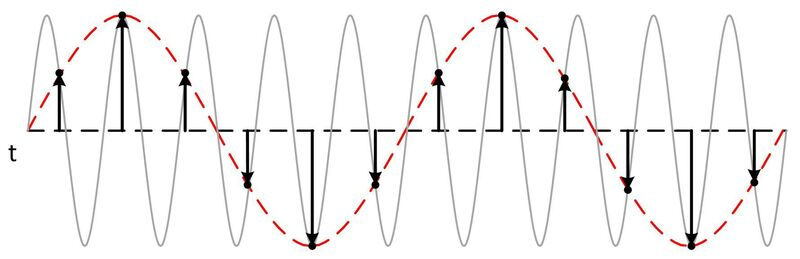
\includegraphics[width=1.0\linewidth,height=50mm]{Abbildungen/grundlagen/abtasttheorem}
		\caption[Originalsignal und durch Abtastung rekonstruiertes Signal]{Originalsignal (grau) und durch Abtastung rekonstruiertes Signal (rot)\, \cite{BBG.2020}
		}
		\label{fig.Abtasttheorem}
	\end{center}
\end{figure}

\section{Wahrscheinlichkeitsverteilungen}
\label{sec.Wahrscheinlichkeitsverteilungen}
% to-do: Einleitung hier reinschreiben. Warum brauchen wir Wahrscheinlichkeitsfunktionen überhaupt?
Dieser Abschnitt behandelt Wahrscheinlichkeitsverteilungen. Wahrscheinlichkeitsverteilungen werden benötigt, um Aussagen über das Ergebnis einer Aktion, wie beispielsweise den Ausgang eines Münzwurfes, zu treffen \cite{Teschl.2014}. Außerdem können mit ihrer Hilfe Aussagen über den Wert von Umweltzuständen für Zeitpunkte getroffen werden, zu denen dieser nicht direkt beobachtbar ist. Diese Aussagen werden dabei mit Hilfe gesammelter Informationen über vergangene Werte des Umweltzustandes getroffen \cite{Krajnik.2015}. Neben der Binomialverteilung wird im Folgenden auch auf die Poissonverteilung eingegangen. 
\subsection{Binomialverteilung}
\label{sec.Binomialverteilung}
% Einleitung zu Binomialverteilung schreiben

Ein Münzwurf mit seinen zwei möglichen Ausgängen \glqq{Kopf}\grqq{} beziehungsweise \glqq{Zahl}\grqq{} stellt ein Bernoulli-Experiment dar. Als Bernoulli-Experiment wird ein Zufallsexperiment bezeichnet, bei dem es lediglich zwei Ausgänge geben kann, ein Ereignis $A$ also entweder eintritt oder nicht \cite{Teschl.2014}. Führt man ein Bernoulli-Experiment $n$ -mal hintereinander unter den gleichen Bedingungen durch, so erhält man eine Bernoulli-Kette der Länge $n \in \mathbb{N}$. Das Eintreten des Ereignisses $A$ wird gemeinhin als Erfolg, die Wahrscheinlichkeit $P(A)=p$ \,  als Erfolgswahrscheinlichkeit bezeichnet \cite{Teschl.2014}. Als Ereignis $A$ kann beispielhaft das Werfen einer Münze mit dem Ausgang \glqq{$Zahl$}\grqq{} genannt werden. Eine Binomialverteilung entsteht, wenn man die Anzahl der Erfolge bei einer Bernoulli-Kette ermitteln will \cite{Teschl.2014}. Mathematisch formuliert lässt sich die Binomialverteilung ausdrücken als
\begin{equation}
	\label{eq:Binomialverteilung}
	P(X=x) = \binom{n}{x} \, p^{x} \, q^{n-x} .
\end{equation}\\
$X$ bezeichnet hierbei die Anzahl der Versuchsdurchführungen, bei denen ein Erfolg eintritt. $X$ kann die Werte $x = 0,1,2,\dots,n$\, annehmen, $p$ steht für die Eintrittswahrscheinlichkeit eines Erfolges, $q$ für die Wahrscheinlichkeit eines Misserfolges. Die Zufallsvariable $X$ ist binomialverteilt und ihre Wahrscheinlichkeitsverteilung eine Binomialverteilung mit den Parametern $n,p$ \cite{Teschl.2014}. Die grafische Darstellung einer Binomialverteilung für die Wahrscheinlichkeit der Anzahl an Würfen eines Würfels mit dem Ereignis \glqq{$1$}\grqq{} bei sieben Würfen ist in \bild{Poisson_Verteilung} dargestellt.

\begin{figure}[!ht]
	\begin{center}
		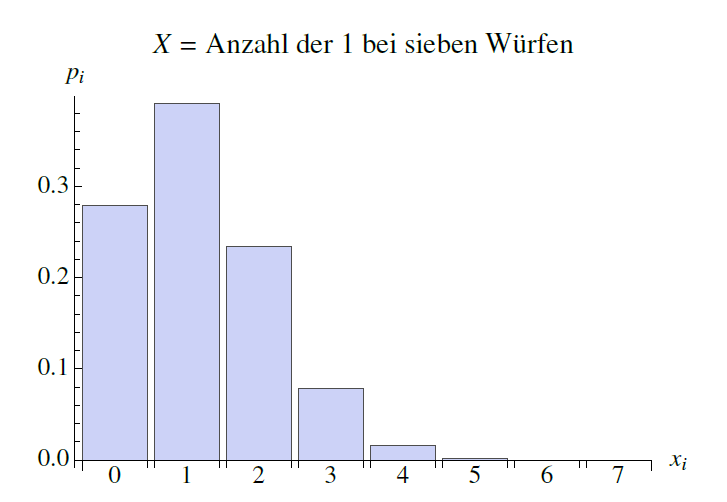
\includegraphics[height=50mm]{Abbildungen/grundlagen/Binomverteilung}
		\caption[Binomialverteilung Beispiel]{Binomialverteilung mit $n = 7, p = \frac{1}{6}$\,  \cite{Teschl.2014}}
		\label{fig.Poisson_Verteilung}
	\end{center}
\end{figure}
\subsection{Poissonverteilung}
\label{sec.Poissonverteilung}
% Einleitung schreiben
Es gibt viele Szenarien, in denen man sich für die Anzahl $X_t$ bestimmter Ereignisse innerhalb eines Zeitraumes interessiert. Beispielhaft können die Anzahl der Verkehrsunfälle pro Tag oder die Anzahl der Fertigungsfehler innerhalb einer Produktionstranche genannt werden \cite{Teschl.2014}. Zur stochastischen Beschreibung dieser Aufgabenstellungen eignet sich die Poisson-Verteilung \cite{Teschl.2014}.
Eine Zufallsvariable $X$, welche unendlich viele Werte $x=0,1,2\dots$ mit den Wahrscheinlichkeiten
\begin{align}
	P(X=x) = \frac{\lambda^{x}}{x!} e^{-\lambda}\qquad  \lambda >0
	\label{eq:Poisson Verteilung}
\end{align}
annehmen kann, wird als poissonverteilt mit dem Parameter $\lambda$ bezeichnet. Die zugehörige Verteilung heißt Poisson-Verteilung. Der Erwartungswert $\mu$ wird beschrieben durch 
\begin{equation}\label{eq:Poisson_EW}
	\mu = E(X) = \lambda ,
\end{equation}
die Varianz $\sigma ^2$ der Poisson-Verteilung berechnet sich zu
\begin{equation}\label{eq:Poisson_Var}
	\sigma^2 = Var(X) = \lambda .
\end{equation}
Anhand der obigen Formeln erkennt man, dass der Parameter der Poisson-Verteilung gleich ihres Erwartungswertes ist, selbiges gilt für die Varianz.
Häufig ist es von Interesse, die Wahrscheinlichkeit für eine Anzahl $X_t$ an Ereignissen innerhalb eines Zeitraumes $[0, t]$ zu bestimmen.
% Ein paar Beispiele nennen
Die Menge von Zufallsvariablen $X_t$ mit $ t\geq 0$ wird als Poisson-Prozess mit der Rate $\lambda$ bezeichnet, falls gilt
\begin{equation}
	P(X_t=x) = \frac{(\lambda t)^x}{x!} e^{-\lambda t} .
	\label{eq:Poisson-Prozess}
\end{equation}
Ein Poisson-Prozess muss dabei nach \cite{Teschl.2014} drei Voraussetzungen erfüllen:
\begin{itemize}
	\item Die Wahrscheinlichkeit für ein Ereignis ist proportional zur Beobachtungsdauer $\Delta t$, aber unabhängig von den Startzeitpunkten, also der zeitlichen Lage des Beobachtungsintervalls.
	\item Die Wahrscheinlichkeiten für ein Ereignis an unterschiedlichen Orten sind voneinander unabhängig.
	\item Für infinitesimal kleine $\Delta t$ ist die Wahrscheinlichkeit, dass das Ereignis mehr als einmal auftritt, im Vergleich zur Wahrscheinlichkeit, dass es genau einmal vorkommt, vernachlässigbar klein \cite{Teschl.2014}.
\end{itemize}

\section{Beschreibung binärer Zustandsmodelle}
\label{sec.Beschreibung binärer Zustandsmodelle}
Mobile Roboter finden immer mehr Einzug in Umgebungen, welche von Menschen bewohnt sind \cite{Krajnik.2017}. Diese Menschen üben Aktivitäten aus, welche in der Folge zu Veränderungen der Umgebung führen. Geht man davon aus, dass viele dieser Aktivitäten täglichen Routinen mit typischen Mustern folgen, kann man probieren, diese zu modellieren. Die Modelle können dann von mobilen Robotern zur robusteren Darstellung ihrer Umgebung genutzt werden. Das Mapping in statischen Umgebungen, also die Kartierung, stellt ein weit erforschtes Gebiet dar \cite{Lakemeyer.2003}.
Für das Mapping dynamischer Umgebungen gibt es verschiedene Ansätze. Während ein Ansatz darauf abzielt, sich bewegende Objekte aus der Umgebungsdarstellung herauszufiltern \cite{Hahnel.2002}, werden in anderen diese Objekte getrackt und als bewegte Landmarken klassifiziert \cite{Montesano.2008}. Diese separationsbasierten Ansätze können jedoch nicht auf Langzeitveränderungen der Umgebungsstruktur reagieren. \\
Im Gegensatz hierzu stehen adaptive Ansätze, welche davon ausgehen, dass der Prozess des Mappings niemals komplett abgeschlossen ist und dieser kontinuierlich aktualisiert werden muss. So können der Karte durch neue Observierungen des mobilen Roboters neue Features hinzugefügt werden 
\cite{Milford.2010}. In \cite{Krajnik.2014} wird versucht, die räumlich-zeitliche Dynamik einer Umgebung durch ihr Frequenzspektrum darzustellen. Die Werte von lokalen Umweltzuständen, wie zum Beispiel einer Tür, welche entweder offen oder geschlossen sein kann, sollen anhand von Wahrscheinlichkeitsfunktionen repräsentiert werden, welche aus der Superposition periodischer Funktionen resultieren. In \cite{Krajnik.2014} wird als Motivation dazu angeführt, dass bei den meisten Mapping-Ansätzen wichtige Umweltzustände lediglich statisch durch zwei eindeutige Zustände dargestellt werden. Eine Tür ist also entweder dauerhaft geöffnet oder geschlossen.
Diese Zustände können jedoch auch durch ihre Wahrscheinlichkeit ausgedrückt werden. Hierbei beschreibt $p_j$ die Wahrscheinlichkeit des $j$-ten Umweltzustandes einer Umgebung. Bayes-Filter gehen hierzu von einer statischen Welt aus, d.h. die Wahrscheinlichkeit des Zustandes $p_j$ wird als konstant angesehen. Durch neue Beobachtungen können diese konstanten Annahmen verändert werden, alte Beobachtungen werden so jedoch über die Zeit \emph{vergessen} \cite{Krajnik.2014}. Nimmt man an, dass diese Zustandswahrscheinlichkeiten $p_j (t)$ Funktionen der Zeit sind und diesen zeitlichen Veränderungen der Wahrscheinlichkeiten eine finite Anzahl periodischer Prozesse zu Grunde liegt, so könnte man den Einfluss und die Periodizität eben dieser Prozesse identifizieren und die Zustandswahrscheinlichkeit $p_j (t)$ aus dieser Beschreibung ermitteln. In \cite{Krajnik.2014} wird die in Abschnitt \ref{sec.Fourierreihen und Fouriertransformation} erläuterte Fouriertransformation benutzt, um diese periodischen Prozesse zu identifizieren. Als Beispiel wird ein Belegungsgitter herangeführt. Jede der Zellen des Belegungsgitters kann zwei Zustände $s_j = \{frei, belegt\}$ annehmen. Diese Zellzustände sind jedoch nicht konstant, sondern eine Funktion $s_j (t) $ der Zeit. Die Unsicherheit des Zustandes wird durch seine Wahrscheinlichkeit $p_j (t)$ ausgedrückt. Da die Zellen als unabhängig voneinander betrachtet werden, kann die Fouriertransformation separat auf jede Zelle des Belegungsnetzes angewendet werden. \\ Die über die Zeit aufgetragenen Zustände einer Zelle $s(t)$ werden mittels der Fouriertransformation $P = FT(s(t))$ transformiert. Es werden \textit{l} Koeffizienten $P_i$ des Spektrums $P$ ausgewählt und zusammen mit ihren Frequenzen $\omega_i$ benutzt, um mittels der inversen Fouriertransformation $p(t) = IFT(P'(t))$ die Wahrscheinlichkeitsfunktion $p(t)$ des Zellzustandes zu bestimmen. Die Menge $P$ besteht hierbei aus einer Anzahl von $l$ Tripeln mit den Einträgen $(abs(P_i), arg(P_i), \omega_i)$, wobei $abs(P_i)$ für die Amplitude, $arg(P_i)$ für den Phasenversatz und $\omega_i$ für die Frequenz des jeweiligen periodischen Prozesses steht, welcher den Zustand $s(t)$ beeinflusst. Anschließend wird ein Schwellwert benutzt, um aus $p(t)$ eine Schätzung $s'(t)$ der tatsächlichen Zustandsfunktion $s(t)$ zu bestimmen. \\

Der Zustand einer Zelle kann somit durch  
\begin{equation}
	s(t) = (IFT(P) > 0.5)
	\label{eq:Zellzustand}
\end{equation}
approximiert werden.

Ist die Wahrscheinlichkeit $p(t)$ einer Zellbelegung größer als 0.5, so wird die Zelle als belegt geschätzt.

Der in Gleichung \ref{eq:Zellzustand} benutzte Schwellwert von 0.5 kann willkürlich gesetzt werden. So können Vorhersagen über zukünftige Zustände der Zelle mit einem gewissen Konfidenzniveau von $c$ durch die Gleichung
\begin{equation}
	s'(t,c) = IFT(P) > c
	\label{eq:Zustandsvorhersage}
\end{equation}
getroffen werden. Diese Methode wird im Folgenden als Frequency Map Enhancement (FreMEn) bezeichnet. Grafisch verdeutlicht wird die Methode durch \bild{FreMEn Beispiel}. 

\begin{figure}[!ht]
	\begin{center}
		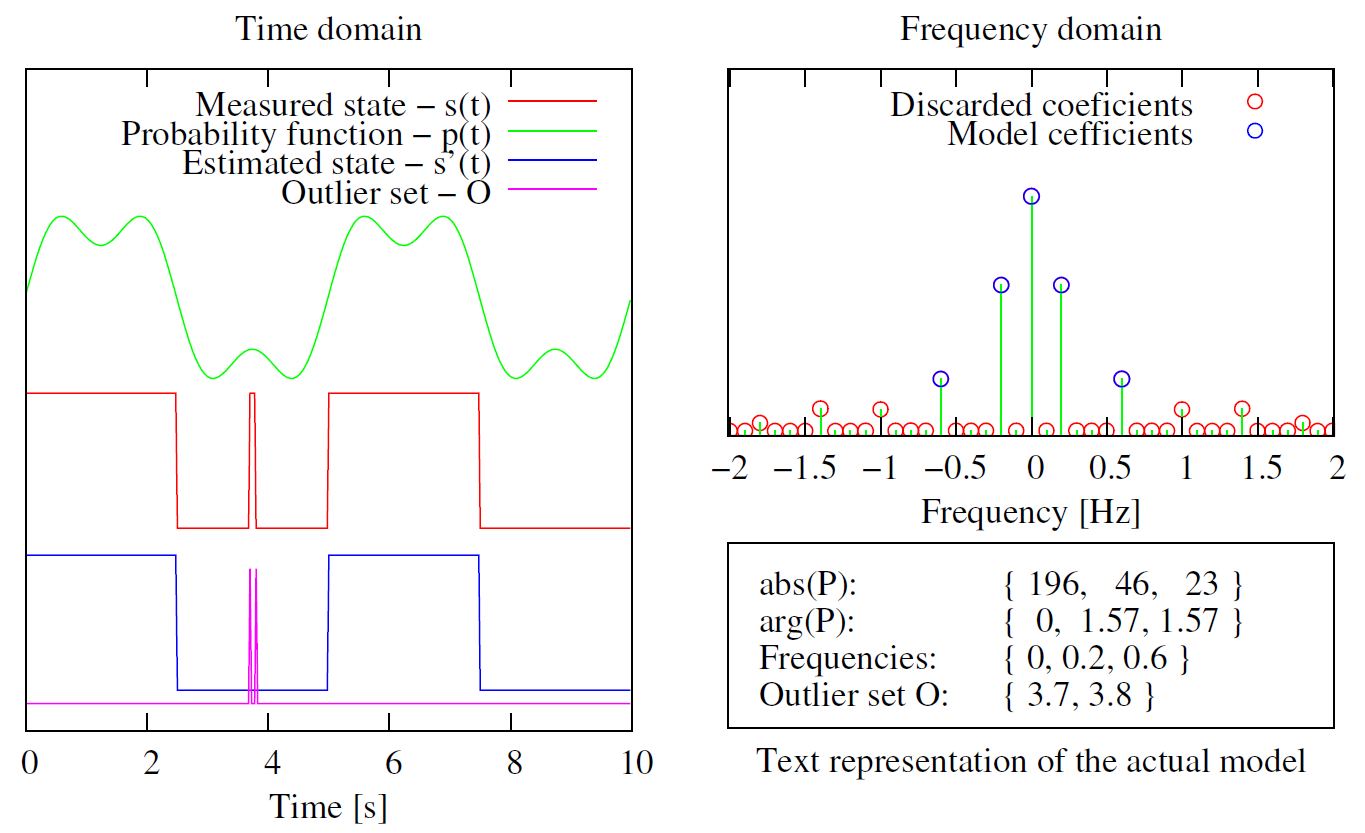
\includegraphics[height=70mm]{Abbildungen/stand_der_technik/example_of_measured_state_and_prediction}
		\caption{Beispiel eines über die Zeit gemessenen Zellzustandes sowie seines Spektralmodells und seiner Wahrscheinlichkeitsprädiktion\, \cite{Krajnik.2014}}
		\label{fig.FreMEn Beispiel}
	\end{center}
\end{figure}
% Outlier-Set beschreiben

In der linken Grafik rot dargestellt sind die, über einen zeitlichen Verlauf aufgenommenen, binären Zustände $s(t)$ einer Beispielzelle. Der grüne Graph beschreibt das zugehörige FreMEn-Modell $p(t)$ der Ordnung $l = 3$. Zur Konstruktion von $p(t)$ wurden somit drei periodische Prozesse verwendet. In blau aufgetragen sind die Vorhersagen $s'(t)$ des Modells, ermittelt anhand eines Schwellwertes von $c = 0.5$ \,. Der lila Graph stellt die Zeitpunkte dar, zu denen die Modellvorhersage von den tatsächlichen Zellzuständen abweicht \cite{Krajnik.2014}. Die rechte obere Grafik repräsentiert das Frequenzspektrum der Zelle, die für das Modell ausgewählten Frequenzen sind durch blaue Kreise markiert. Das zuvor erwähnte Tripel bestehend aus Amplitude, Phasenversatz und Frequenz der jeweiligen periodischen Prozesse ist in der rechten unteren Grafik dargestellt. Daneben findet sich hier auch die Menge der Ausreißer $\mathcal{O}$ mit den Zeitpunkten, zu denen die Modellvorhersage $s'(t)$ von den tatsächlichen Zellzuständen $s(t)$ abweicht.  Um die Auswirkungen des Modellgrades, also der Anzahl der in das Modell einfließenden periodischen Prozesse, zu erforschen, wurde die Methode auf einen Datensatz angewendet, bei welchem ein mobiler SCITOS-G5 Roboter, ausgestattet mit RGB-D und Lasersensoren, Personen in einem Bürogebäude über eine Dauer von einer Woche mit einer Frequenz von \SI{30}{\hertz} detektiert hat. \\
Die Genauigkeit des Modells $q(t_a,t_b)$ wird berechnet als
\begin{equation}
	q(t_a,t_b) = \frac{1}{t_b - t_a} \int_{t_a}^{t_b} |s'(t) - s(t)| \ind{d}t
	\label{eq:Modellgenauigkeit}
\end{equation}
und beschreibt das Verhältnis von korrekt geschätzten Zellzuständen zu der Gesamtdauer des betrachteten Intervalls.

Unterschieden wird in \cite{Krajnik.2014} nun zwischen der Rekonstruktionsgenauigkeit $q_\ind{r}$ sowie der Prädiktionsgenauigkeit $q_\ind{p}$. Die Rekonstruktionsgenauigkeit beschreibt, wie genau das Modell Zeitintervalle beschreibt, welche zur Ermittlung der Modellparameter verwendet wurden. Die Prädiktionsgenauigkeit hingegen beschreibt die Genauigkeit des Modells in Bezug auf Zeiträume, welche nicht zur Modellermittlung verwendet wurden. Die ermittelte Abhängigkeit der Rekonstruktions-sowie Prädiktionsgenauigkeit von der Modellordnung $l$ ist in \bild{predict_reconstruct_error} aufgezeigt. Hierbei erfolgte die Berechnung des Modells und der Rekonstruktionsgenauigkeit $q_\ind{r}$ anhand eines einwöchigen Datensatzes, die Evaluierung des Modells und die Ermittlung der Prädiktionsgenauigkeit $q_\ind{p}$ wurde mittels zwei externer Tage mit den zugehörigen Prädiktionsgenauigkeiten $q_\ind{p1}$ und $q_\ind{p2}$ durchgeführt.  \\

\begin{figure}[!ht]
	\begin{center}
		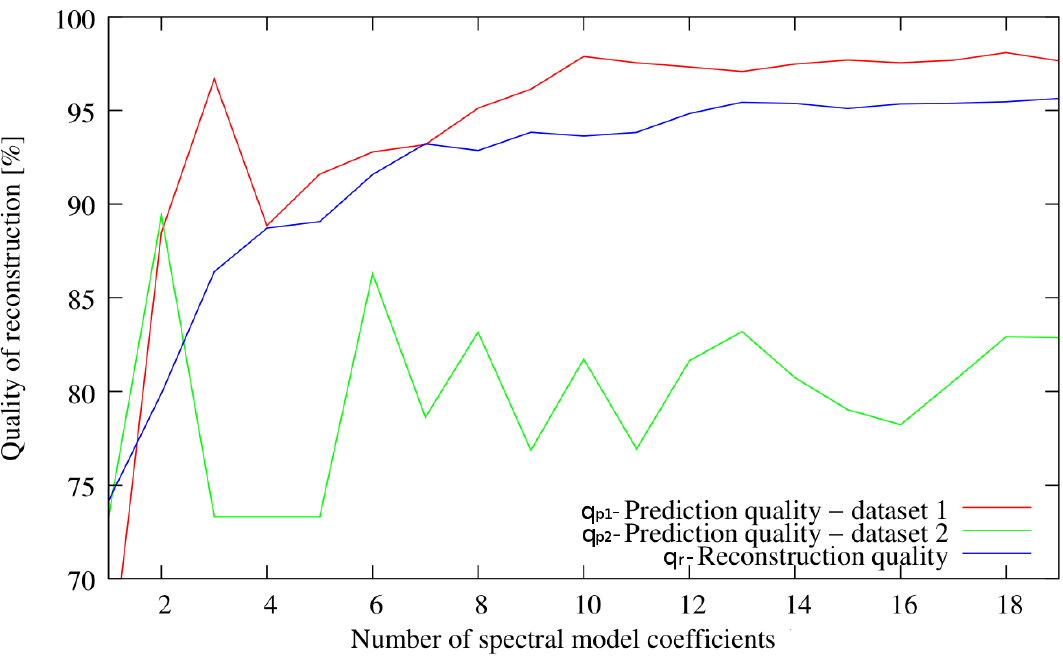
\includegraphics[width=0.7\linewidth]{Abbildungen/stand_der_technik/predict_reconstruct_error}
		\caption{Modellgenauigkeit vs. Modellordnung\,\cite{Krajnik.2014}}
		\label{fig.predict_reconstruct_error}	
	\end{center}
	
\end{figure}

Die Rekonstruktionsgenauigkeit liegt bei einer Modellordnung von $l=15$, d.h. es wurden 15 periodische Prozesse zum Approximieren des Zustandssignales verwendet, bei 95 \%. Die Rekonstruktionsgenauigkeit $q_\ind{r}$ steigt dabei monoton mit der Modellordnung. Für die Prädiktionsgenauigkeit $q_\ind{p}$ lässt sich nach \cite{Krajnik.2014} kein allgemeingültiger Zusammenhang finden. Während die Prädiktionsgenauigkeit des ersten Testtages bei $l=3$ ein lokales Maximum, bei $l=17$ jedoch ein globales Maximum besitzt, liegt das globale Maximum für den zweiten Testtag bei $l=2$.\\
Die lokalen Maxima von $q_\ind{p1}$ und $q_\ind{p2}$ lassen laut \cite{Krajnik.2014} den Schluss zu, dass für die Vorhersage eine Modellordnung von zwei oder drei optimal ist (siehe \bild{predict_reconstruct_error}). \\
Einen Vergleich zwischen der in \cite{Krajnik.2014} beschriebenen FreMEn- Methode und der Anwendung von periodischen Gauß-Mischmodellen zur Darstellung der Dynamik von binären Umweltzuständen zieht \cite{Krajnik.2015b}. FreMEn basiert hier, wie auch schon in \cite{Krajnik.2014} auf der Idee, die zeitliche Funktion $s(t)$ eines Umweltzustandes durch seine Wahrscheinlichkeitsfunktion $p(t)$ zu schätzen. Auch hier wird wieder mittels einer Fouriertransformation das Frequenzspektrum $S(\omega)$ der zeitlichen Funktion $s(t)$ bestimmt, und die \textit{l} prominentesten Frequenzen mit ihren Amplituden $a_j$, ihrem Phasenversatz $\varphi_j$ sowie ihrer Frequenz $\omega_j$ abgespeichert. Die Ermittlung der Wahrscheinlichkeit $p(t)$ eines Umweltzustandes zum Zeitpunkt \textit{t} ergibt sich durch die Superposition der \emph{l} Frequenzen zu
\begin{equation}
	p(t) = a_0 + \sum_{j=1}^{n} a_j \cos(\omega_j t + \varphi_j) .
	\label{eq:Superposition}
\end{equation}
Die erste spektrale Komponente $a_0$ stellt hierbei den Durchschnitt aller binären Werte von $s(t)$, also dessen Gleichanteil (siehe Abschnitt \ref{sec.Fourierreihen und Fouriertransformation}) dar. FreMEn besitze aber laut \cite{Krajnik.2015b} zwei wesentliche Nachteile. So erlaube es zum einen, lediglich einen periodischen Prozess pro Frequenz zu modellieren. Des Weiteren bilde es wiederkehrende, aber kurze, Prozesse schlecht ab. Als Beispiel wird hier die morgendliche Dusche angeführt, welche eine tägliche, aber kurze Routine sei. Da in \cite{Krajnik.2014} herausgearbeitet wurde, dass die optimale Modellordnung $l_\ind{opt}$ für eine möglichst hohe Prognostiziergenauigkeit bei einer Größe von lediglich zwei bis drei liegt, könnten solche kurzen Routinen nicht abgebildet werden. \\ Als zweiter Ansatz werden Gaussian Mixture Models (GMM) genannt. Diese können multidimensionale Funktionen als gewichtete Summe aus mehreren Gauß-Funktionen durch
\begin{equation}
	f(t) = \frac{1}{\sqrt{2 \pi}} \sum_{j=1}^{m} \frac{\omega_j}{\sigma_j} e^{- \frac{(t- \mu_j)^2}{2 \sigma_j ^2}}
	\label{eq:Gaussian_Mixture_Models}
\end{equation}
approximieren.
Die Parameter der individuellen Komponenten eines GMM, namentlich das Gewicht $\omega_j$, der Durchschnitt $\mu_j$ sowie die Standardabweichung $\sigma_j$ werden typischerweise mittels Trainingsdaten anhand des Iterative Expectation Maximization (EM) oder des Maximum A-Posteriori (MAP) Algorithmus ermittelt. Während GMM in der Lage sind, Funktionen jeglichen Aussehens zu modellieren, liegt ihre Limitation darin, dass sie definitionsgemäß keine periodischen Funktionen repräsentieren können \cite{Krajnik.2015b}. Um diesem Problem entgegenzuwirken, wird vorab eine Periodendauer von einem Tag vorgegeben. Diese Vorgabe erlaubt es, die gemessene Sequenz der Umweltzustände $s(t)$  in eine Sequenz $p'(t)$ umzuwandeln mit
\begin{equation}
	p'(t) = \frac{k}{\tau} \sum_{i=1}^{\frac{k}{\tau}} s(t+i \tau) .
	\label{eq:GMM_sequence}
\end{equation}
In Gleichung (\ref{eq:GMM_sequence}) bezeichnet $\tau$ die vorab definierte Periodendauer, $k$ beschreibt die Länge der Sequenz $s(t)$. Nach Anwendung des Expectation Maximization Algorithmus kann die Wahrscheinlichkeit für einen Umweltzustand berechnet werden zu
\begin{equation}
	p(t) = \frac{1}{\sqrt{2 \pi}} \sum_{j=1}^{m} \frac{w_j}{\tau_j} e ^{- \frac{(mod(t,\tau) - \mu_j)^2}{2 \sigma_j^2}} .
	\label{eq:Gauss_Probability}
\end{equation}
Hierbei beschreibt $\tau$ die vorgegebene Periodendauer der Funktion $p(t)$ und $mod$ ist der Modulo-Operator. Dass die Stärken und Schwächen dieser periodischen GMM-basierten (PerGaM) Modelle komplementär zu jenen der FreMEn-Methodik sind, wir anhand von \bild{PerGaM_vs_FreMEn} deutlich.
\begin{figure}[!ht]
	\begin{center}
		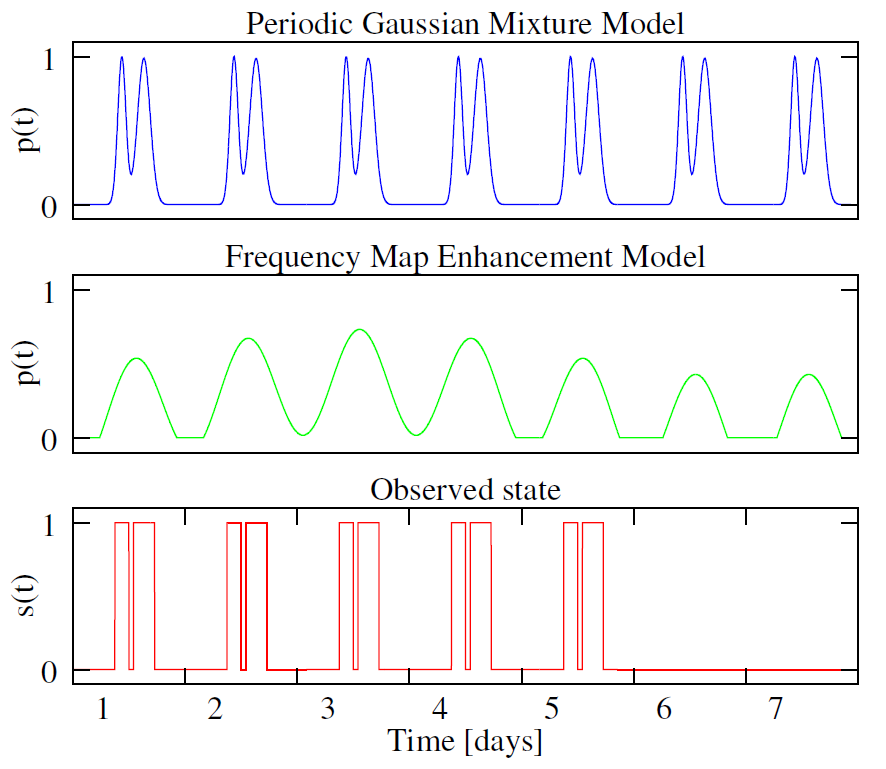
\includegraphics[width=0.7\linewidth]{Abbildungen/stand_der_technik/PerGaM_vs_FreMEn}
		\caption{PerGaM und FreMEn Modellvergleich\, \cite{Krajnik.2015b}}
		\label{fig.PerGaM_vs_FreMEn}
	\end{center}
\end{figure}
Das PerGaM-Modell kann selbst kurze, mehrfach auftretende Routinen approximieren, jedoch kann es lediglich eine Periodendauer repräsentieren, welche a priori bekannt bzw. festgelegt werden muss. Als Resultat werden kurzzeitige Routinen, wie z.B. Mittagspausen, gut approximiert, die wöchentliche Dynamik mit dem Fehlen von Personen am Wochenende kann hingegen nicht modelliert werden. Im Vergleich dazu sieht man das FreMEn-Modell, welches die Wochendynamik durch ein Abflachen der Signalamplitude an den beiden Wochenendtagen abbildet (siehe \bild{PerGaM_vs_FreMEn}). \\
In Bezug auf das zeitlich-räumliche Mapping durch mobile Roboter führt \cite{Krajnik.2015} an, dass dies auch eine räumlich-zeitliche Explorationsstrategie benötigt. Im Vergleich zu klassischen Explorationsstrategien, bei denen, bedingt durch die endliche Größe der zu erforschenden Karte, die Exploration ebenfalls finit ist, sei die Exploration dynamischer Umgebungen niemals abgeschlossen. Vielmehr würde die räumlich-zeitliche Exploration Teil der täglichen Routine des Roboters werden.
Es stellt sich ein wesentlicher Nachteil der in \cite{Krajnik.2014} vorgestellten Methode zur Darstellung von binären Umweltzuständen in Bezug auf die kontinuierliche Exploration einer Karte durch einen mobilen Roboter heraus. Diese beruht auf der traditionellen Fast Fourier Transformation (FFT). Die Fast Fourier Transformation kann jedoch lediglich die komplette Sequenz eines Umweltzustandes $s(t)$ in sein Frequenzspektrum $S(\omega)$ transformieren. Außerdem erfordert der Algorithmus, dass die Zustandsobservierungen mit der immer gleichen Frequenz aufgenommen werden.  Orte mit der immer selben Frequenz zu erkunden, sei jedoch nicht effizient, sodass in \cite{Krajnik.2015} eine neue Methode zur Darstellung von binären Umweltzuständen durch zeitlich variable Wahrscheinlichkeitsfunktionen vorgestellt wird. Die Methode erlaubt ein inkrementelles und kontinuierliches Aktualisieren des räumlich-zeitlichen Umgebungsmodells durch wenige Observierungen, welche zu unterschiedlichen, nicht gleichmäßig verteilten Zeitpunkten, und an unterschiedlichen Orten aufgenommen werden können. \\
Jeder Umweltzustand $s(t)$ wird durch die Anzahl getätigter Observierungen $n$, seines Durchschnittes $\mu$ sowie zwei Sets $A,B$ komplexer Zahlen $\alpha_k$ und $\beta_k$, welche zu dem Set $\Omega$ periodischer Prozesse $\omega_k$ gehören, die den Umweltzustand beeinflussen, beschrieben. Anfangs wird der Wert $\mu$ jedes Umweltzustandes zu $\mu = 0.5$ und alle $\alpha_k$ sowie $\beta_k$ zu 0 gesetzt, was einem vollkommen unbekannten Zustand entspricht. Die inkrementelle Aktualisierung des Modells erfolgt durch 
\begin{align}
	\mu &\leftarrow \frac{1}{n+1}(n \mu + s(t)), \\
	\alpha_k &\leftarrow \frac{1}{n+1} (n \alpha_k + s(t) e^{-jt\omega_k}) ,  &\forall \omega_k \in \Omega, \\
	\beta_k &\leftarrow \frac{1}{n+1} (n \beta_k + \mu e^{-jt\omega_k}) ,  &\forall \omega_k \in \Omega, \\
	n &\leftarrow n + 1 .
	\label{eq:Update_step_FreMEn}
\end{align}
Die schrittweise Aktualisierung entspricht dabei einer inkrementellen Mittelwertbildung. Der Betrag $\gamma_k = |\alpha_k - \beta_k|$ stellt den durchschnittlichen Einfluss des periodischen Prozesses $k$ auf den Umweltzustand $s(t)$ dar.
Wären die Zeitpunkte $t$ der Observationen und die Frequenzen $\omega_k$ gleichmäßig verteilt, so entsprächen die obigen Formeln der diskreten Fouriertransformation.
Um den zukünftigen Wert eines Umweltzustandes prognostizieren zu können, werden wie auch in \cite{Krajnik.2014} die $m$ periodischen Prozesse mit den höchsten absoluten Werten $|\gamma_k|$ ausgewählt. Die Wahrscheinlichkeit eines Umweltzustandes wird mittels
\begin{equation}
	p(t) = \varsigma(\mu + \sum_{l=1}^{m} |\gamma_l|\cos(\omega_k t + arg(\gamma_l)))
	\label{eq:State_probability}
\end{equation}
berechnet. Die Funktion $\varsigma(.)$ sorgt dafür, dass $p(t) \in [0,1]$ gilt. Der optimale Wert für $m$ wird wie schon in \cite{Krajnik.2014} so gewählt, dass die Prädiktionsgenauigkeit $q_\ind{p}$ maximiert wird. \\

\section{Beschreibung quantitativer Zustandsmodelle}
\label{sec.Beschreibung quantitativer Zustandsmodelle}
% Einleitung quantitativer Zustandsmodelle
Aus Abschnitt \ref{sec.Beschreibung binärer Zustandsmodelle} wurde ersichtlich, dass
binäre Zustandsmodelle Aussagen über die Wahrscheinlichkeit $p(t)$ eines Zellzustandes, wie z.B. die Belegtheit einer Zelle $s(t)$, erlauben. Möchte man jedoch Schätzungen für die Anzahl, wie oft eine Zelle innerhalb eines Zeitintervalls belegt bzw. besucht wird, treffen, so ist dies nur durch eine quantitative Zustandsbeschreibung möglich.
Eine Methode zur Modellierung von quantitativen Umweltzuständen wird in \cite{Jovan.2016} vorgestellt. Die hier genannte Methode beruht auf der Kombination von zeitveränderlichen Poisson-Prozessen und einer Frequenzanalyse. Dabei wird die Häufigkeit des Auftretens eines Ereignisses innerhalb eines Zeitintervalls gezählt. Anders ausgedrückt wird gezählt, wie häufig ein Umweltzustand, beispielsweise das Vorhandensein einer Person in einer Zelle, den Wert \emph{wahr} pro Zeitintervall annimmt. Somit kann anstatt der Wahrscheinlichkeitsfunktion $p(t)$ eines Umwelt- bzw. Zellzustandes dessen Intensität bzw. Rate innerhalb des Zeitintervalls dargestellt werden. Diese Raten $\lambda (t)$ werden mit Hilfe von Poisson-Prozessen modelliert. Wie schon  in Abschnitt \ref{sec.Poissonverteilung} beschrieben, wird auch hier die Poisson-Verteilung mittels
\begin{equation}
	P(N;\lambda) = \frac{e^\ind{-\lambda} \lambda^N}{N!}, \qquad	N=0,1,2,\dots
\end{equation}

berechnet, wobei $P(N;\lambda)$ die Wahrscheinlichkeit $P$ für den Fall beschreibt, dass innerhalb eines Zeitintervalls $\Delta t_i$ mit einer durchschnittlichen Aktivitätenanzahl, also einer durchschnittlichen Personenanzahl von $\lambda$, exakt $N$ Aktivitäten, also Personen, gezählt werden. Die Daten in \cite{Jovan.2016} wurden von einem mobilen Metralabs Scitos A5-Roboter aufgenommen, welcher sich, ausgestattet mit einem robusten Personen-Tracking-Algorithmus, einen Monat lang in einem Bürogebäude bewegte. Die Abhängigkeit der durchschnittlichen Personenanzahl $\lambda$ vom betrachteten Zeitintervall wird durch $\lambda (t_i, t_j)$ ausgedrückt, wobei  $t_i$ den Anfangszeitpunkt und $t_j$ den Endzeitpunkt des Intervalls beschreibt. Da die von dem Roboter aufgenommenen Daten nur einen kleinen Teil der Gesamtheit des Personenaufkommens repräsentieren, wird $\lambda$ mittels einer Konfidenz-basierten Schätzung bestimmt. Der Poisson-Parameter $\lambda$ folgt hierbei einer Gammaverteilung
\begin{equation}
	\lambda \sim \Gamma(\lambda ; \alpha, \beta) .
\end{equation}
Die a-posteriori Wahrscheinlichkeit für $\lambda (t_i, t_j)$ berechnet sich unter Berücksichtigung der aufgenommenen Daten zu
\begin{equation}
	P(\lambda | x_1, \dots, x_n) = \Gamma(\lambda, \alpha + \sum_{i=1}^{n} x_i, \beta +n) ,
\end{equation}
wobei $x_1, \dots , x_n$ die im betreffenden Intervall aufgezeichneten Daten bezeichnen, der Parameter $\alpha$ steht für den Formfaktor, $\beta$ für den inversen Skalenparameter der Gammaverteilung.
Der Datensatz wird in Wochen eingeteilt, für ein Zeitintervall wird eine Dauer von zehn Minuten gewählt. Die Maximum a posteriori-Wahrscheinlichkeit (MAP) jedes Parameters $\lambda(t_i, t_j)$ wird als Punktschätzung für $\lambda$ gewählt. Die Verknüpfung sämtlicher Punktschätzungen über den definierten Zeitraum einer Woche ergibt das Poisson-Prozess-Modell, welches in \bild{poisson-prozess-model1} grafisch aufgezeichnet ist. 
\begin{figure}[!ht]
	\begin{center}
		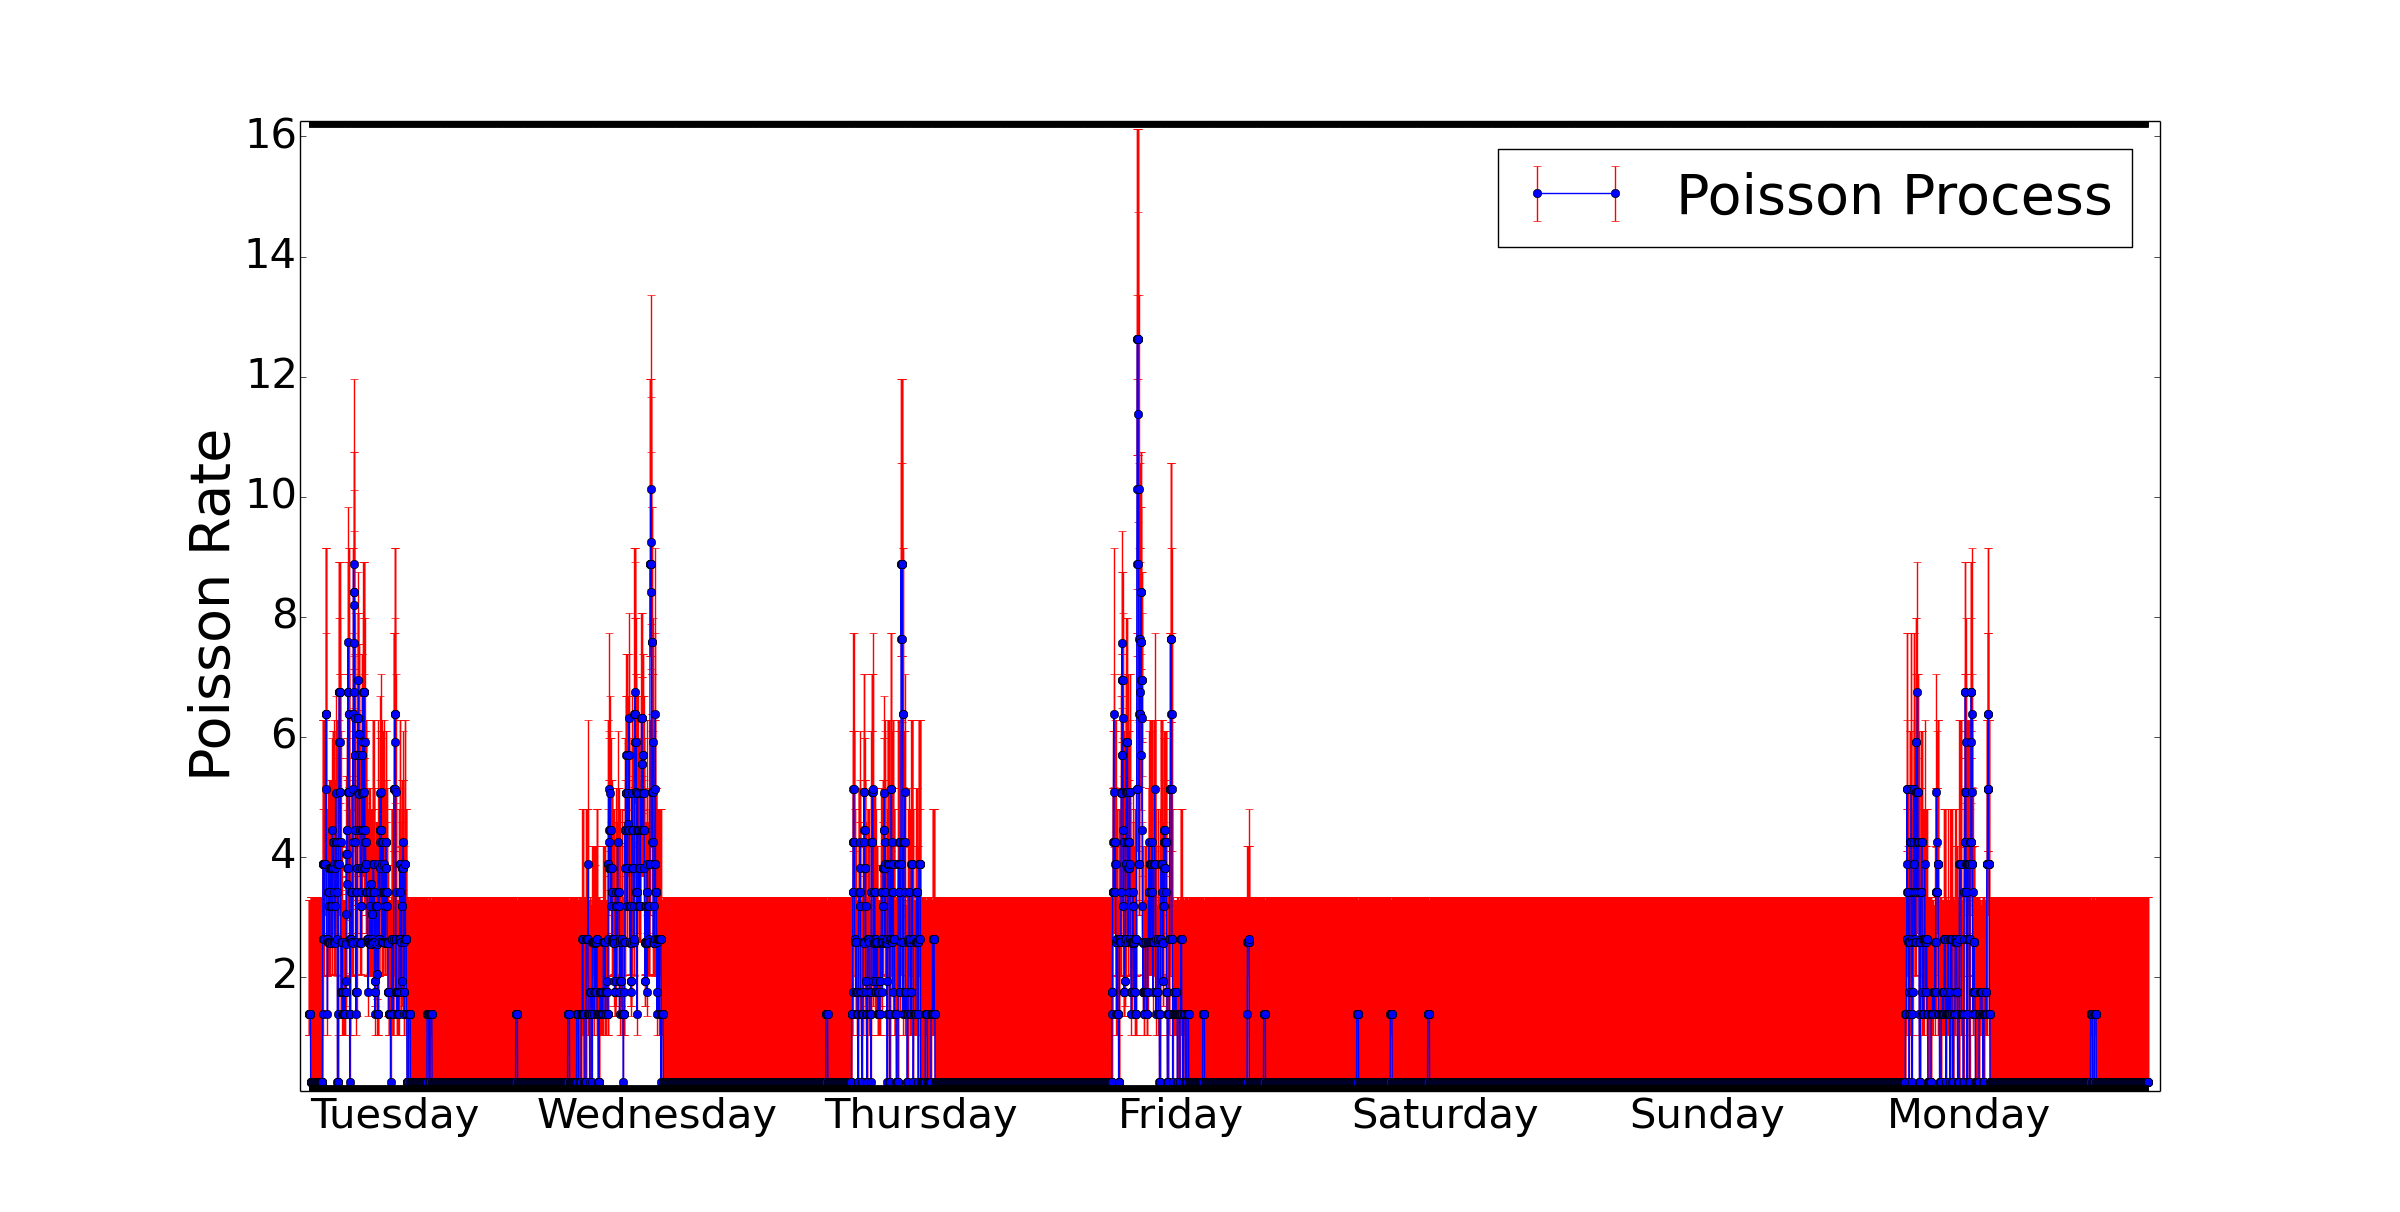
\includegraphics[width=0.8\linewidth]{Abbildungen/stand_der_technik/poisson-prozess-model1}
		\caption{Aktivitätsraten $\lambda$ des Poisson-Prozess-Modells ermittelt anhand eines 4 Wochen Zeitraumes\, \cite{Jovan.2016}}
		\label{fig.poisson-prozess-model1}
	\end{center}
\end{figure}

Für jedes $\lambda$ wurden die Daten von vier aufeinanderfolgenden Wochen verwendet, die roten Schranken zeigen die oberen und unteren Grenzen des Konfidenzintervalls für jedes $\lambda$. \\
Nach der Berechnung des Poisson-Prozess-Modells wird nun die Fouriertransformation auf $\lambda (t)$ angewendet. Ebenso wie in \cite{Krajnik.2014} werden die $l$ Frequenzen mit den höchsten Amplituden zur Konstruktion von $\lambda' = IFT(F'(\omega))$ verwendet. Im Gegensatz zu der in \cite{Krajnik.2014} durch Superposition der Parameter der $l$ prominentesten Frequenzen verwendeten und hier als \emph{l Best Amplitude Model} (BAM) bezeichneten Methode wird in \cite{Jovan.2016} die \emph{l Addition Amplitude Model} (AAM) Methode verwendet. Es wird angeführt, dass das BAM den Betrag des Original-Signals nicht komplett abbilden kann, sofern die Sampling-Rate der Daten deutlich höher ist als die höchste beobachtete Frequenz. \\ AAM hingegen berechnet das Fourierspektrum des Poisson-Prozess-Modells, findet die Frequenz $\omega_k$ mit der höchsten Amplitude und zieht es von den Daten ab. Die modifizierten Daten werden wieder transformiert und das Frequenzspektrum erneut berechnet. Findet sich in diesem Frequenzspektrum eine bereits vorher identifizierte Frequenz, so wird dessen neuerliche Amplitude auf die bereits vorhandene addiert, und die Daten erneut modifiziert. Dieses Vorgehen wird bis zur Identifikation der $l$ Frequenzen mit den höchsten Amplituden wiederholt. \bild{BAM_AAM_Vergleich} bietet einen Vergleich der beiden Methoden zur Abbildung des Poisson-Prozess-Modells. Aus der Grafik wird ersichtlich, dass das AAM die Beträge des Original-Modells deutlich besser abbilden kann als das BAM.

\begin{figure}[!ht]
	\centering
	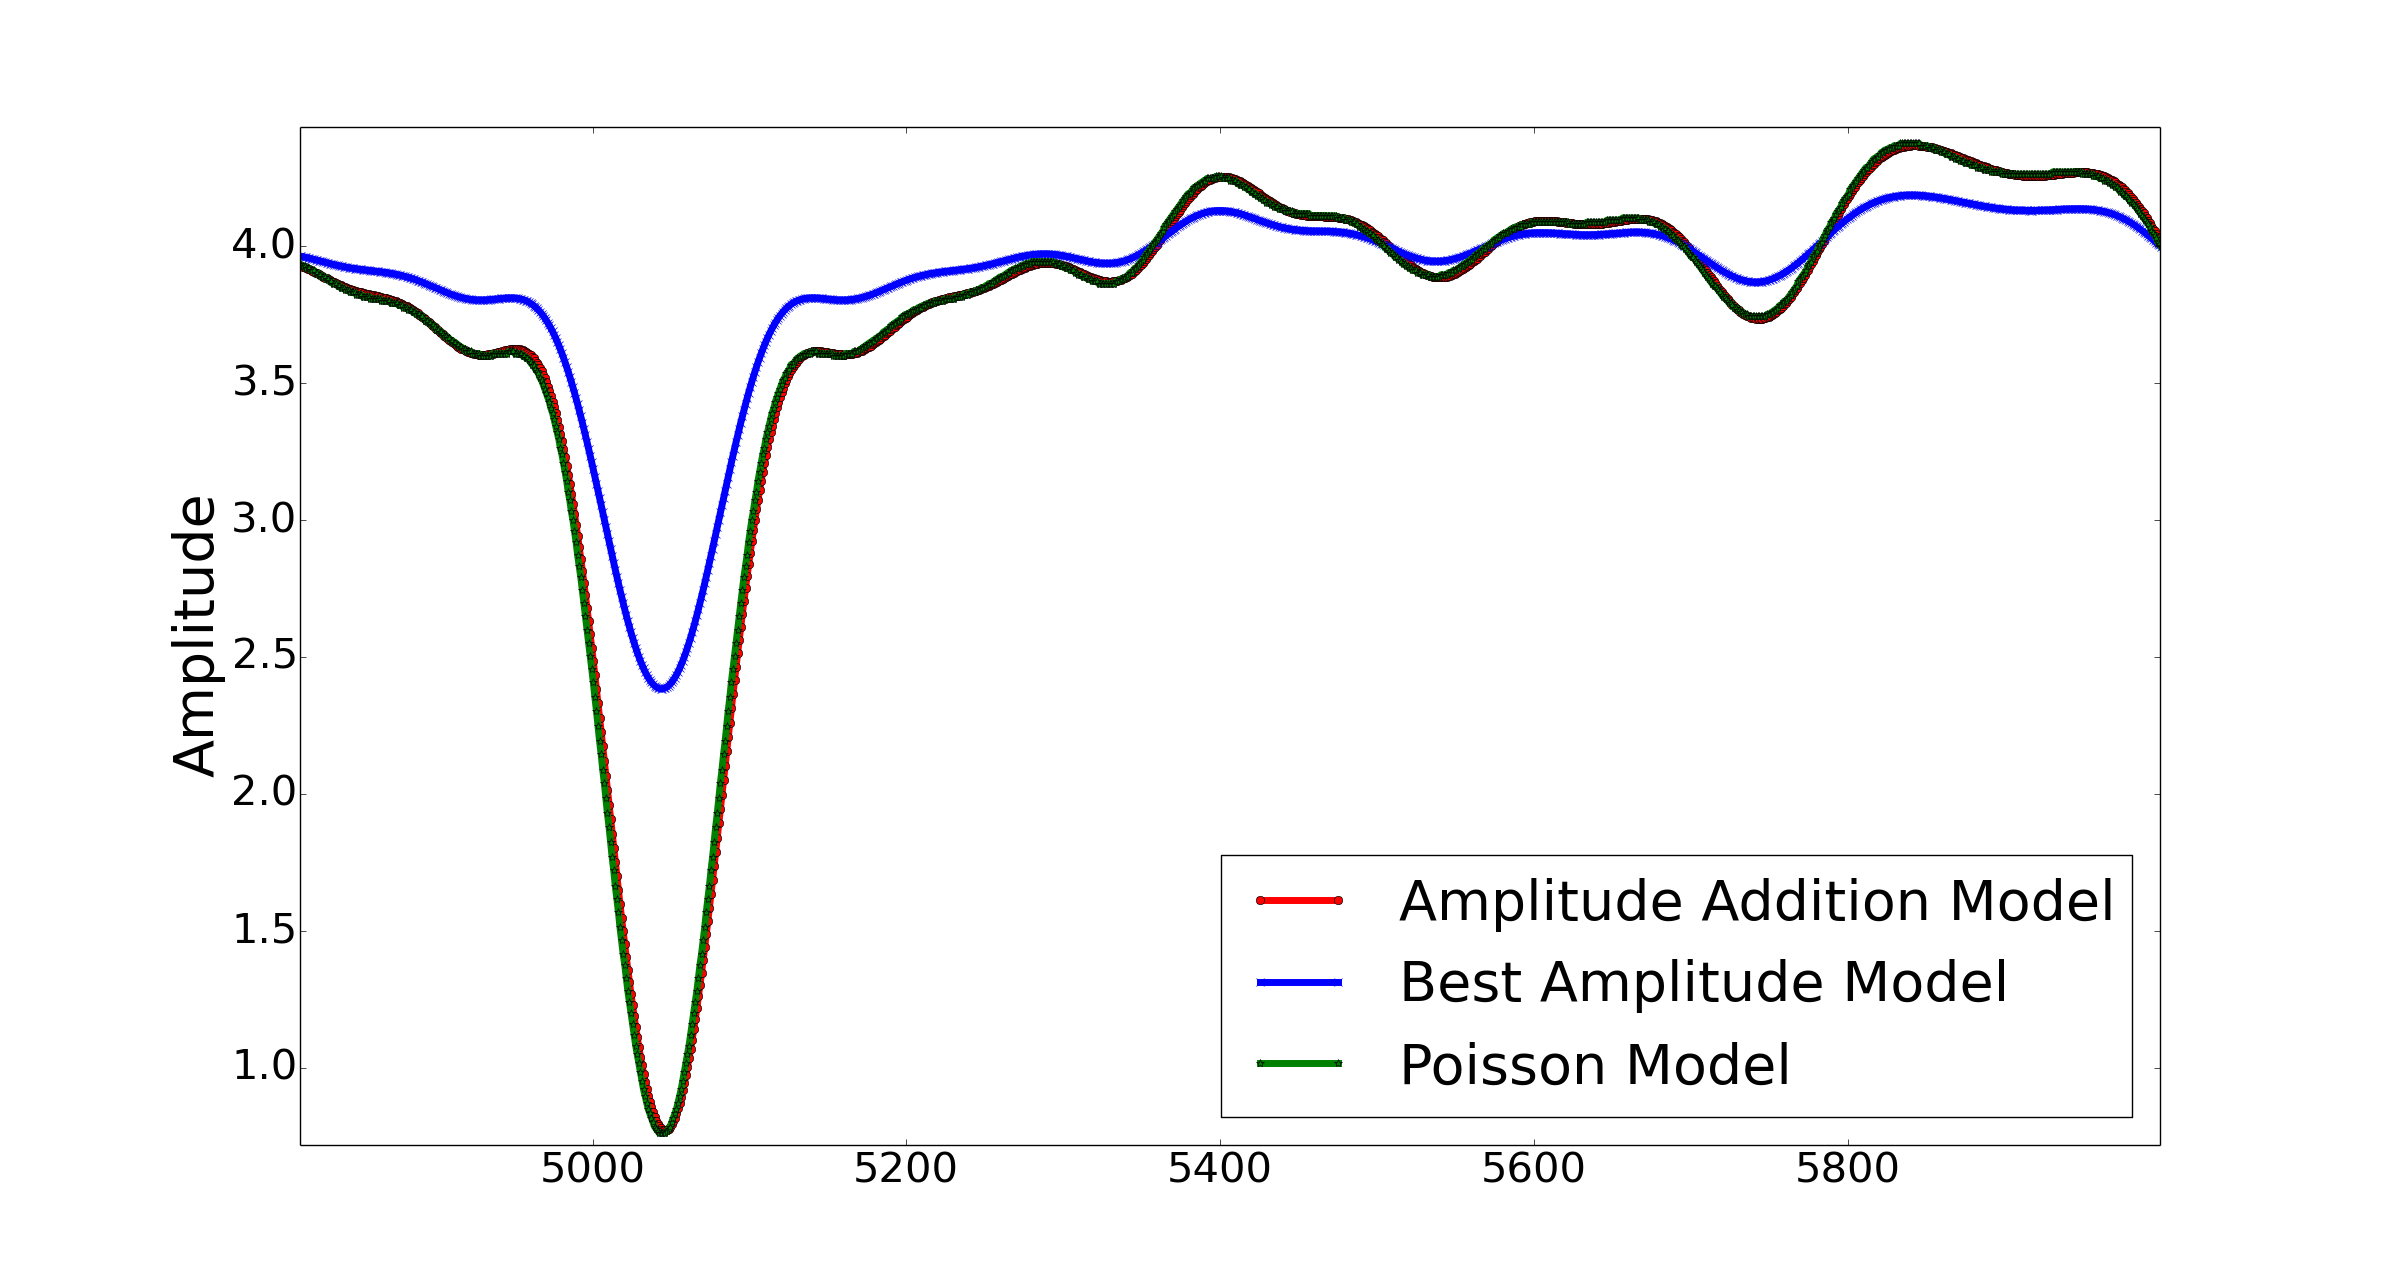
\includegraphics[width=0.8\linewidth]{Abbildungen/stand_der_technik/BAM_AAM}
	\caption{Vergleich \emph{l Best Amplitude Model} und \emph{l Addition Amplitude Model} \, \cite{Jovan.2016}}
	\label{fig.BAM_AAM_Vergleich}
\end{figure}

Eine genauere Beschreibung der Berechnung des Formfaktors $\alpha$ und des inversen Skalenparameters $\beta$ der Gammafunktion findet sich in \cite{Stuede.2020}. Hier wird der Parameter $\lambda$ für jede Zelle eines 2D-Gitters berechnet. Die Wahrscheinlichkeit
für die Anzahl $N$ an Aktivitäten innerhalb eines Zeitintervalls in einer Zelle des Gitters kann dargestellt werden über
\begin{equation}
	P_{ij \tau} (N(t) = k) = \frac{(\lambda_{ij \tau}(t-t_\tau))^k}{k!} e^{-\lambda_{ij\tau} (t- t_\tau)} ,
\end{equation}
wobei $\lambda_{ij \tau}$ für die Rate an Aktivitäten der Zelle $(i,j)$ innerhalb des Zeitintervalls $\tau$ steht. Die der Zelle und dem jeweiligen Intervall zugehörigen Parameter $\alpha_{ij\tau}$ sowie $\beta_{ij\tau}$ werden inkrementell für jeden Zeitschritt $\sigma$ bestimmt  mittels der Vorschrift
\begin{equation}
	\alpha_\sigma = \alpha_{\sigma - 1} + x_\sigma \boldsymbol{1}_\ind{\mathcal{D}} (\boldsymbol{x}_\ind{R}, t_\sigma),\qquad  \beta_\sigma = \beta_{\sigma - 1} + \boldsymbol{1}_\ind{\mathcal{D}} (\boldsymbol{x}_\ind{R}, t_\sigma ) .
\end{equation}
Als Anfangswerte werden $\alpha_0 = \beta_0 = 1 $ gewählt. Die Indikator-Funktion $\boldsymbol{1}_\ind{\mathcal{D}} (\boldsymbol{x}_r, t_\sigma)$ resultiert hierbei aus dem Detektionsbereich eines Roboters bei der Pose $\boldsymbol{x}_\ind{R}$. Die a-posteriori erwarteten Werte der Aktivitätenrate $\lambda$ und ihrer Varianz berechnen sich für jedes Intervall zu
\begin{equation}
	\hat{\lambda}_{ij\tau} = E[\lambda_{ij\tau}] = \frac{\alpha_{ij\tau}}{\beta_{ij}\tau},\qquad	Var[\lambda_{ij\tau}] = \frac{\alpha_{ij\tau}}{\beta_{ij\tau}^2} .
\end{equation}


